% !TeX root = ../main.tex
\documentclass[class=article]{standalone}

\begin{document}
\section*{Question 6}

Dérivation à gauche d'abord.
\begin{deriv}
    S
    \<\lmdev
    \commentaire{S $\rightarrow$ aSbSa}
    aSbSa
    \<\lmdev
    \commentaire{S $\rightarrow$ $\epsilon$}
    abSa
    \<\lmdev
    \commentaire{S $\rightarrow$ bSaSa}
    abbSaSaa
    \<\lmdev
    \commentaire{S $\rightarrow$ $\epsilon$}
    abbaSaa
    \<\lmdev
    \commentaire{S $\rightarrow$ $\epsilon$}
    abbaaa
\end{deriv}

\bigskip

Dérivation à droite d'abord.
\begin{deriv}
    S
    \<\rmdev
    \commentaire{S $\rightarrow$ aSbSa}
    aSbSa
    \<\rmdev
    \commentaire{S $\rightarrow$ bSaSa}
    aSbbSaSaa
    \<\rmdev
    \commentaire{S $\rightarrow$ $\epsilon$}
    aSbbSaaa
    \<\rmdev
    \commentaire{S $\rightarrow$ $\epsilon$}
    aSbbaaa
    \<\rmdev
    \commentaire{S $\rightarrow$ $\epsilon$}
    abbaaa
\end{deriv}

\pagebreak

Arbre de dérivation

\begin{tikzpicture}
    [
    every leaf node/.style={draw,circle},
    sibling distance=2em, level distance=40pt]

    \tikzset{edge from parent/.style={draw, edge from parent path=
    {(\tikzparentnode) -- (\tikzchildnode)}}}
    \Tree 
    [.S 
        a
        [.S
            $\epsilon$
        ]
        b
        [.S 
            b 
            [.S
                $\epsilon$
            ] 
            a 
            [.S
                $\epsilon$
            ]
            a
        ]
        a
    ]
\end{tikzpicture}


\end{document}